\documentclass[11pt,a4paper]{article}

\usepackage[T1]{fontenc}
\usepackage[utf8]{inputenc}
\usepackage{lmodern}
\usepackage{amsmath,amssymb}
\usepackage{graphicx}
\usepackage{xcolor}
\usepackage{booktabs}
\usepackage{hyperref}
\usepackage{microtype}
\usepackage{geometry}
\geometry{margin=1in}

\hypersetup{
  colorlinks=true,
  linkcolor=blue!60!black,
  citecolor=blue!60!black,
  urlcolor=blue!60!black
}

\title{%
  MEEP-Gated Search on DRC Manifolds for\\
  Silicon 1$\times$2 Power Splitters
}
\author{Petr Berlizov\\
  Harvard University}
\date{June 2026}

\begin{document}
\maketitle

\begin{abstract}
We study a reproducible search \emph{pattern} for DRC-feasible silicon 1$\times$2 splitters: sample on a generative manifold, rank with a lightweight surrogate, and promote only MEEP-verified layouts under a frozen forward-model contract (\texttt{phase0\_v1}).
The primary gate is a balanced upper-arm fraction $R_{\mathrm{up}} \approx 0.50$ at 1550\,nm ($|R_{\mathrm{up}}-0.5|\le 0.05$); every reported number uses the same 2D TE recipe on 180$\times$180 masks in a 4\,$\mu$m design region.

In a six-seed pilot at matched MEEP budgets $B\in\{30,50,100\}$, surrogate-ranked search yields the highest mean verified in-spec count at $B{=}100$ ($15.7\pm 3.3$ of $B$) and the lowest mean best split error ($0.0037\pm 0.0030$), with paired wins 4/6 vs.\ $\sigma$-only MEEP BO and a 3/6 tie vs.\ hierarchical $\sigma$-search---evidence that ranking concentrates simulation dollars on better split candidates, not a statistically definitive policy ordering ($n{=}6$).
The pipeline finds in-spec layouts both near and far from a published reference in pixel space; a rank-gated round promotes \texttt{cand\_000261} at $R_{\mathrm{up}}=0.4946$ with mesh-audit cross-checks.

We do \emph{not} claim deployment-ready splitters, low insertion loss, C-band WDM flatness, or morphology robustness under fabrication stress.
Release diagnostics document why: single-$\lambda$ promotion does not imply 1530--1570\,nm flatness (0/39 verified candidates pass); promoted masks fail binary $\pm 10$--$20$\,nm morphology gates (0/517 refine trials pass); flux-monitor transmission stays low ($T_{\mathrm{total}}\sim 0.01$--$0.03$, IL$\sim 15$--$19$\,dB, uncalibrated to foundry loss).
Those negative results bound the present recipe and motivate the adoption roadmap in \S\ref{sec:roadmap}.
\end{abstract}

\section{Introduction}
\label{sec:intro}

C-band 1$\times$2 power splitters are routine building blocks in silicon photonic integrated circuits (PICs)~\cite{LalauKranz2013Splitters,Joannopoulos2011Waveguides}, yet verifying a tight 50/50 ratio under a fixed forward model remains sensitive to geometry details that adjoint optimizers and hand-tuned templates handle unevenly~\cite{Piggott2017InverseDesign,Hammond2022MeepAdjoint}.
A layout that appears balanced in one simulation setup can miss the target split in another, because the mask-to-split map is nonlinear and strongly tied to port placement, polarization assumptions, and mesh resolution~\cite{Piggott2017InverseDesign}.
This sensitivity motivates a \emph{search-and-verify} pipeline that (i)~restricts candidates to fabrication-feasible masks, (ii)~spends a limited MEEP budget wisely, and (iii)~reports all numbers under one frozen forward-model contract so that comparisons are internally consistent.
We treat device performance beyond the split gate---broadband flatness, insertion loss, morphology tolerance---as separate engineering targets documented in release diagnostics, not as claims of this study~\cite{Hansen2024BroadbandSplitters,Piggott2017FabricationConstrained}.

MEEP adjoint topology optimization~\cite{Oskooi2010Meep,Hammond2022MeepAdjoint} can sculpt free-form devices, yet still requires a fixed port template and explicit fabrication constraints.
Recent DRC manifolds~\cite{Danis2026DRCManifold} encode feasible layouts by construction, removing a class of mask violations before simulation.
They do not, by themselves, settle which forward solver and mesh recipe should sign off a design---a question that matters because promotion criteria and surrogate labels must refer to the same physics.

Neural surrogates~\cite{Jiang2021SurrogateReview,Su2021DeepSurrogate} and Bayesian search loops~\cite{Shahriari2016BO,Freitas2020BO,SciRep2025CNNIBO,MAPS2025} are often evaluated on holdout regression $R^2$.
In our corpus, however, most labels are far from 50/50, so $R^2$ is a weak gate: a model can rank poorly on absolute error while still surfacing useful shortlists.
What matters for a fixed MEEP budget is whether ranked proposals yield more in-spec masks than random or $\sigma$-only search when the same number of forward simulations is spent.

We fix one MEEP recipe (\texttt{phase0\_v1}) and stay on it for labeling, surrogate training, promotion, and budget comparisons.
Latents decode through Danis \emph{et al.}'s EBeam model~\cite{Danis2026DRCManifold}; sampling mixes local $\sigma$ moves, MEEP-guided Optuna, and Perlin seeds far from the published template.
A mask MLP with pairwise rank loss~\cite{Burges2010LambdaRank} pre-filters candidates; MEEP verifies and promotes.
Promoted layouts must also pass a dual-resolution mesh check on \texttt{phase0\_v1\_sdf\_geom}, so that split claims are not artifacts of a single pixel grid.
Six search policies are compared at matched MEEP budgets over six independent seeds---a pilot replication, not a definitive policy ranking.

\paragraph{Contributions.}
This preprint is a methods starting point, not a device datasheet.
We claim:
\begin{enumerate}
  \item A reproducible MEEP-gated loop on a DRC-feasible manifold: sample $\to$ surrogate rank $\to$ MEEP verify $\to$ corpus, with open artifacts under \texttt{data/phase0/} and \texttt{data/phase1/}.
  \item Pilot evidence ($n{=}6$ seeds) that surrogate-ranked search improves \emph{verified} 50/50 split-ratio yield per simulation dollar vs.\ random perturbation and $\sigma$-only MEEP BO at $B{=}100$, with paired-win accounting.
  \item Honest diagnostic negatives under the same contract: narrowband promotion $\neq$ C-band flatness; promoted masks are morph-fragile under pixel stress; flux-monitor IL and $T$ remain poor and uncalibrated to foundry insertion loss.
\end{enumerate}
We do \emph{not} claim low-loss or broadband WDM-ready splitters, morphology-robust designs, foundry-calibrated IL, or statistically definitive ordering of search policies.

Separately, we run invrs-gym Ceviche benchmarks~\cite{Christiansen2024InvrsGym,Fan2019Ceviche,Schubert2022CevicheChallenges} as an external FDFD sanity check on gradient flow through the decoder.
Those numbers are informative but not interchangeable with the MEEP contract, and we treat them as a parallel track rather than a replacement for promotion gates.

\section{Problem and forward-model contract}
\label{sec:problem}

Before describing search, we define the device target, geometry template, and frozen MEEP recipe that govern every label and promotion decision in this work.
Keeping this contract explicit is essential: without it, split ratios from different simulators, resolutions, or port templates cannot be compared meaningfully.

\subsection{Device and figure of merit}

We target a 50/50 power splitter at the C-band center wavelength $\lambda_0 = 1550$\,nm.
The primary scalar figure of merit is the upper-arm power fraction
\begin{equation}
  R_{\mathrm{up}} = \frac{P_{\mathrm{up}}}{P_{\mathrm{up}} + P_{\mathrm{low}}}
\end{equation}
monitored in the upper output arm.
A design is \emph{in-spec} if $|R_{\mathrm{up}} - 0.5| \le 0.05$, i.e., within five percentage points of a balanced split.
Secondary metrics---total transmission, insertion loss, and C-band split flatness---are logged throughout; we report them in \S\ref{sec:release_checks} but do not use them as hard promotion gates in Phase~0, because monitor calibration and broadband objectives remain open engineering items.

\subsection{Geometry template}

Every candidate mask is 180$\times$180 binary pixels on a 4\,$\mu$m $\times$ 4\,$\mu$m design island centered in a 6\,$\mu$m $\times$ 6\,$\mu$m unit cell.
Input and output Si strip waveguides attach at fixed ports ($w_g = 0.45\,\mu\mathrm{m}$ in the production recipe).
The template therefore defines a 1$\times$2 splitter topology regardless of how the generative model was trained.
Labels are self-consistent within this frozen frame, not absolute comparisons to arbitrary published FDTD setups~\cite{Piggott2017InverseDesign}.

\subsection{Production recipe \texttt{phase0\_v1}}

Table~\ref{tab:recipe} lists the production settings; Appendix~\ref{app:recipe} has the full parameter table.
Several choices materially affect how a given mask maps to $R_{\mathrm{up}}$:
\begin{itemize}
  \item 2D TE (\texttt{Ez}) with $\varepsilon_{\mathrm{Si}} = 12$, $\varepsilon_{\mathrm{SiO}_2} = 2.25$.
  \item Resolution 25\,px/$\mu$m; Gaussian line source at $f = 1/1.55\,\mu\mathrm{m}^{-1}$.
  \item \texttt{mask\_flip\_y=true}: without flip, the published reference splits $\sim$0.33/0.67 in-template; with flip, $R_{\mathrm{up}} \approx 0.61$.
\end{itemize}
The \texttt{mask\_flip\_y} flag is part of the contract, not a universal physical correction: it aligns the decoded mask orientation with the fixed port frame used here.

This recipe is \emph{frozen} for corpus labeling, surrogate training, and promotion.
Any change requires a new \texttt{recipe\_version} column; historical rows are not retroactively relabeled, so that surrogate training and budget comparisons remain tied to a stable forward model.

\begin{table}[t]
  \centering
  \caption{Core \texttt{phase0\_v1} parameters.}
  \label{tab:recipe}
  \begin{tabular}{ll}
    \toprule
    Parameter & Value \\
    \midrule
    Recipe ID & \texttt{phase0\_v1} \\
    Polarization & 2D TE (\texttt{Ez}) \\
    Resolution & 25\,px/$\mu$m \\
    Cell / design region & 6\,$\mu$m / 4\,$\mu$m \\
    Mask grid & 180$\times$180 \\
    \texttt{mask\_flip\_y} & \texttt{true} \\
    In-spec criterion & $|R_{\mathrm{up}} - 0.5| \le 0.05$ \\
    \bottomrule
  \end{tabular}
\end{table}

\subsection{Reference layout under the frozen contract}

We import a published reference latent (\texttt{ref\_published}) through the same decode path used for all search candidates.
Under \texttt{phase0\_v1}, it yields $R_{\mathrm{up}} \approx 0.614$---not in-spec---despite being a reasonable starting point in the broader inverse-design literature.
The result underscores that the mask-to-split map is nonlinear and tied to this template: a layout that looks balanced elsewhere can miss 50/50 here, and any search baseline must be evaluated under the same recipe rather than assumed from prior publications.

\subsection{Expert $\sigma$-perturbation baseline}

To quantify how hard local tuning is on the manifold, we use random $\sigma$-scaled perturbations around \texttt{ref\_published} as a stand-in for expert hand-tuning.
We draw $n{=}100$ such perturbations and measure both geometric distance from the reference and split performance.
Mean pixel Hamming distance from the reference is 3.44\% (95th percentile 5.72\%), yet only 3/100 land in-spec ($\sim$3\%).
In-spec perturbations differ by at least 2.0\% Hamming; the champion \texttt{local\_00022} differs by only 0.47\% yet hits $R_{\mathrm{up}} = 0.500$.
Small geometric edits can therefore flip the split by $\sim$0.11 while blind $\sigma$ tuning rarely finds 50/50---a pattern that motivates structured search beyond local perturbations alone.

\section{Search pipeline}
\label{sec:pipeline}

Figure~\ref{fig:pipeline} sketches the overall loop: sample on the DRC-feasible manifold, rank with a surrogate, verify shortlisted candidates in MEEP, and append verified labels to the corpus.
The surrogate reduces the number of expensive forward simulations required to encounter good designs, but MEEP remains the sole authority for promotion.

\subsection{DRC-feasible manifold}

We use the external \texttt{drcgenerator} package with EBeamModel~\cite{Danis2026DRCManifold}.
Each latent vector $\mathbf{z}$ decodes to a binary 180$\times$180 mask satisfying heuristic EBL design rules (minimum width/spacing on the training manifold).
We do not run end-to-end differentiable manifold optimization as in Danis \emph{et al.}; instead, we borrow their decoder as the feasible search space, ensuring that every candidate mask is manufacturable under the model's rules before simulation.

Sampling modes cover both local refinement and exploration far from the published template:
\begin{description}
  \item[$\sigma$-local.] Gaussian perturbations around known latents (\texttt{ref\_published}, champions), mimicking incremental expert edits.
  \item[MEEP BO.] Optuna-driven $\sigma$ search with MEEP-evaluated objectives~\cite{Freitas2020BO}, spending simulation budget on promising local regions.
  \item[Perlin far-manifold.] Structured latent seeds exploring regions not reachable by small $\sigma$ edits from the published template.
\end{description}
Together, these modes let the pipeline both polish near-reference layouts and discover topologically distinct masks that a single-reference workflow would unlikely reach.

\subsection{Surrogate pre-filter (ranking, not sign-off)}

Because MEEP dominates runtime, we train a lightweight mask MLP that maps decoded masks (plus optional $\sigma$ features) to a scalar score for pre-filtering.
Training uses MEEP labels from \texttt{sim\_results\_phase0\_v1\_all.csv} ($>3600$ ok rows after merges).
Two loss modes were compared to understand whether absolute regression or relative ordering better supports shortlist construction:
\begin{itemize}
  \item \textbf{Regression (MSE):} holdout $R^2 \approx -0.51$; val Spearman on $|R_{\mathrm{up}}-0.5|$ $\approx 0.38$.
  \item \textbf{Pairwise rank (\texttt{surrogate\_improved\_rank}):} $R^2 \approx -19$ on val (worse, expected); Spearman $\approx 0.50$--$0.73$ depending on corpus snapshot; wins \texttt{ranking\_eval} against random top-$k$.
\end{itemize}

Negative $R^2$ is expected in this regime: most labels lie far from 50/50, so predicting absolute split error is ill-conditioned.
The model's job is instead to sort $M \gg B$ proposals cheaply and let MEEP spend its budget on the top $B$.
It never promotes a design on its own.

Ranking evaluation on 3695 held-out rows (top-$k=20$) confirms the intended behavior: surrogate top-$k$ mean $|R_{\mathrm{up}}-0.5| = 0.059$ vs.\ random $0.221$; 13 vs.\ 1 in-spec in top-20 (\texttt{ranking\_wins=true}).
In other words, the surrogate concentrates MEEP calls on layouts that are closer to balanced, even when it cannot predict $R_{\mathrm{up}}$ accurately in an $R^2$ sense.

\subsection{MEEP-gated shortlist rounds}

Each acquisition round follows the same MEEP-gated protocol:
\begin{enumerate}
  \item Train or reload \texttt{surrogate\_improved\_rank}.
  \item Generate $M=500$ on-manifold proposals (\texttt{generate\_ranked\_candidates.py}).
  \item Rank by surrogate score; build MEEP manifest for top 15.
  \item Run \texttt{phase0\_v1} at 25\,px/$\mu$m; append ok rows to corpus.
\end{enumerate}
Only designs verified in MEEP can become champions; the surrogate influences which masks receive that verification.

The lead round (\texttt{round\_rank}, seed 2033) produced champion \texttt{cand\_000261} with $R_{\mathrm{up}} = 0.4946$, improving on prior regression- and $\sigma$-local winners under the same recipe.

\subsection{Sim-budget policies}

To compare search strategies fairly, we implement six policies at matched MEEP budgets $B \in \{30,50,100\}$:
\begin{description}
  \item[\texttt{random\_perturb.}] $B$ random DRC-pass $\sigma$-perturbations, all MEEP-verified.
  \item[\texttt{sigma\_meep.}] $B$ trials of MEEP-guided Optuna on $\sigma$.
  \item[\texttt{surrogate\_rank.}] $M$ proposals ranked; MEEP top $B$.
  \item[\texttt{hierarchical\_35/50/65.}] Fraction $f$ of $B$ on $\sigma$ search, remainder on surrogate-ranked local search around the best $\sigma$ find ($f=0.35,0.50,0.65$).
\end{description}
Six completed replicates use seeds 3026--8026; corpus and surrogate weights are frozen between replicates.
This design isolates policy differences from label drift: every method sees the same forward-model contract and training data snapshot.
We report paired seed wins alongside means because $n{=}6$ is insufficient for strong statistical claims about policy ordering.

\begin{figure}[t]
  \centering
  
\includegraphics[width=\linewidth]{figures/pipeline_schematic.pdf}
  \caption{MEEP-gated search pipeline. The surrogate narrows candidates; MEEP is the sole promotion authority.}
  \label{fig:pipeline}
\end{figure}

\section{Results}
\label{sec:results}

We organize results around three questions: whether MEEP-gated search finds verified split champions under the frozen contract, whether promoted designs are structurally distinct from the reference, and whether surrogate-ranked policies improve verified yield per MEEP call in a six-seed pilot.

\subsection{Champions and MEEP-gated rank round}

Table~\ref{tab:champions} lists representative promoted designs under \texttt{phase0\_v1}.
The rank-surrogate round (\texttt{round\_rank}) improves on prior regression and $\sigma$-local champions, showing that ranking-trained shortlists translate into better verified candidates rather than merely better holdout metrics.

\begin{table}[t]
  \centering
  \caption{Selected champions @ \texttt{phase0\_v1}, $R_{\mathrm{up}}$ at 25\,px/$\mu$m.}
  \label{tab:champions}
  \begin{tabular}{lccc}
    \toprule
    ID & Category & Hamming vs ref & $R_{\mathrm{up}}$ \\
    \midrule
    \texttt{ref\_published} & reference & 0\% & 0.614 \\
    \texttt{local\_00022} & $\sigma$-local & 0.47\% & 0.500 \\
    \texttt{meep\_bo\_00093} & MEEP BO & 0.78\% & 0.497 \\
    \texttt{meep\_bo\_00128} & MEEP BO & 1.00\% & 0.509 \\
    \texttt{cand\_000003} & prior promoted & --- & 0.4902 \\
    \texttt{cand\_000258} & regression r5 best & --- & 0.4886 \\
    \textbf{\texttt{cand\_000261}} & \textbf{rank round} & --- & \textbf{0.4946} \\
    \bottomrule
  \end{tabular}
\end{table}

For \texttt{cand\_000261}, $|R_{\mathrm{up}} - 0.5| = 0.0054$, beating \texttt{cand\_000003} ($0.0098$) and regression round-5 best \texttt{cand\_000258} ($0.0114$).
The top three MEEP-verified proposals from \texttt{round\_rank} were \texttt{cand\_000261} (0.4946), \texttt{cand\_000029} (0.4849), and \texttt{cand\_000004} (0.4765).
Taken together, the round demonstrates that spending only 15 MEEP calls on a surrogate-ranked shortlist can outperform earlier promotion rounds that used regression-based selection.

\subsection{Structural novelty and Hamming distances}

Hamming distance from \texttt{ref\_published} provides a simple geometric notion of ``how different'' a champion is from the published template.
The mask$\to$split map is nonlinear: champions can be \emph{closer} to the reference in Hamming distance than typical random perturbations yet far better in $R_{\mathrm{up}}$.
Conversely, far-manifold Perlin in-spec designs differ by $\sim$51\% Hamming (mean 51.09\%, 95th percentile 55.92\%, $n=24$), outside the expert $\sigma$ ball ($\lesssim$6\%).
Figure~\ref{fig:hamming} shows the cumulative Hamming distribution for $\sigma$-perturb and in-spec Perlin populations.

\begin{figure}[t]
  \centering
  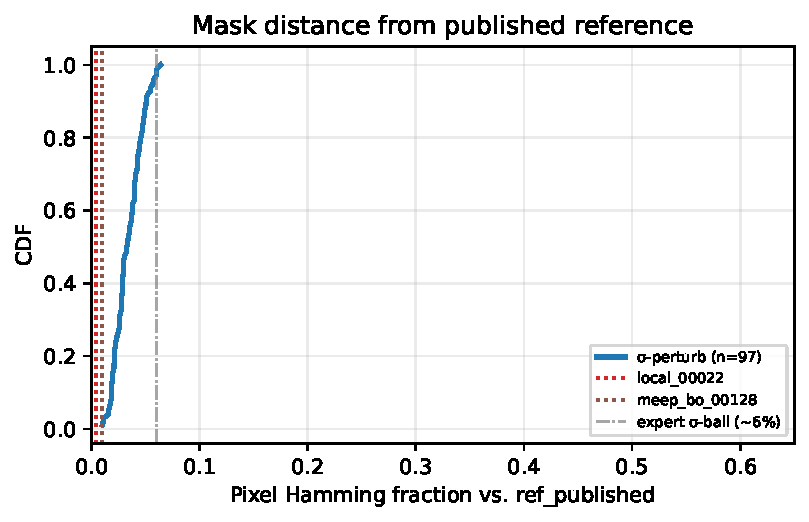
\includegraphics[width=0.92\linewidth]{figures/hamming_cdf.pdf}
  \caption{CDF of pixel Hamming distance vs.\ \texttt{ref\_published} for $\sigma$-perturb samples (all and in-spec subset) and in-spec Perlin samples. Vertical lines mark champions \texttt{local\_00022} and \texttt{meep\_bo\_00128}; the dotted rule at 6\% marks the expert $\sigma$-perturbation ball.}
  \label{fig:hamming}
\end{figure}

The $\sigma$-local winners are small edits of the published mask, not unrelated topologies---they represent the regime where incremental tuning can succeed.
At the same time, in-spec Perlin samples sit far from the template in Hamming space, occupying regions a single-reference tuning workflow is unlikely to reach.
Both regimes yield usable 50/50 candidates under the frozen contract, which suggests the search space contains multiple qualitatively different routes to the same split target.

\subsection{Regression vs.\ ranking surrogate}

On identical corpora, pairwise rank training raises Spearman on $|R_{\mathrm{up}}-0.5|$ from $\sim$0.71 (MSE baseline) to $\sim$0.73 (rank model snapshot), at the cost of worse raw $R^2$ and fewer in-spec in surrogate top-20 on some snapshots (13 vs.\ 5).
Holdout $R^2$ therefore favors the regression model, while shortlist quality favors ranking---a tension resolved only by MEEP verification.
The MEEP-gated \texttt{round\_rank} round is the decisive test: the best verified candidate beats regression-selected champions.
In practice we train for ordering under a fixed MEEP budget, not for val $R^2$.

\subsection{Sim-budget replication}

Table~\ref{tab:budget100} aggregates six replicates at $B=100$, the budget at which policy differences become most visible.
At this budget, \texttt{surrogate\_rank} yields the highest mean in-spec count ($15.7 \pm 3.3$), overlapping with \texttt{hierarchical\_35} ($14.2 \pm 3.5$; paired seed wins 3/6) and ahead of \texttt{sigma\_meep} ($9.8 \pm 4.7$; paired wins 4/6).
\texttt{random\_perturb} ($12.8 \pm 1.6$) and \texttt{hierarchical\_65} ($11.2 \pm 5.8$) sit between.
Mean best $|R_{\mathrm{up}}-0.5|$ is lowest for \texttt{surrogate\_rank} ($0.0037 \pm 0.0030$), overlapping with \texttt{hierarchical\_35} ($0.0046 \pm 0.0031$).
With only six seeds, we treat these as pilot evidence that surrogate ranking concentrates MEEP budget on better split candidates, not as a definitive ranking of hierarchical policies.

At $B=30$, all policies are weak ($\sim$3--4 in-spec mean); we do not draw strong conclusions there, because none of the methods reliably finds balanced splits with so few forward simulations.
At $B=50$, \texttt{hierarchical\_35} leads on count ($9.0 \pm 3.4$) while \texttt{surrogate\_rank} still wins on best error ($0.0064 \pm 0.0057$), suggesting that policy ranking can depend on whether one prioritizes yield or best-single-design quality.

Figure~\ref{fig:budget} plots in-spec yield vs.\ $B$ with error bars, visualizing how performance scales as the MEEP budget increases.

\begin{table}[t]
  \centering
  \caption{Sim-budget replication at $B=100$ (mean $\pm$ std, $n=6$ seeds).}
  \label{tab:budget100}
  \begin{tabular}{lcc}
    \toprule
    Policy & In-spec count / $B$ & Best $|R_{\mathrm{up}} - 0.5|$ \\
    \midrule
    \texttt{surrogate\_rank} & $\mathbf{15.7 \pm 3.3}$ & $\mathbf{0.0037 \pm 0.0030}$ \\
    \texttt{hierarchical\_35} & $14.2 \pm 3.5$ & $0.0046 \pm 0.0031$ \\
    \texttt{random\_perturb} & $12.8 \pm 1.6$ & $0.0060 \pm 0.0055$ \\
    \texttt{hierarchical\_50} & $12.8 \pm 4.1$ & $0.0070 \pm 0.0057$ \\
    \texttt{hierarchical\_65} & $11.2 \pm 5.8$ & $0.0075 \pm 0.0068$ \\
    \texttt{sigma\_meep} & $9.8 \pm 4.7$ & $0.0073 \pm 0.0063$ \\
    \bottomrule
  \end{tabular}
\end{table}

\begin{figure}[t]
  \centering
  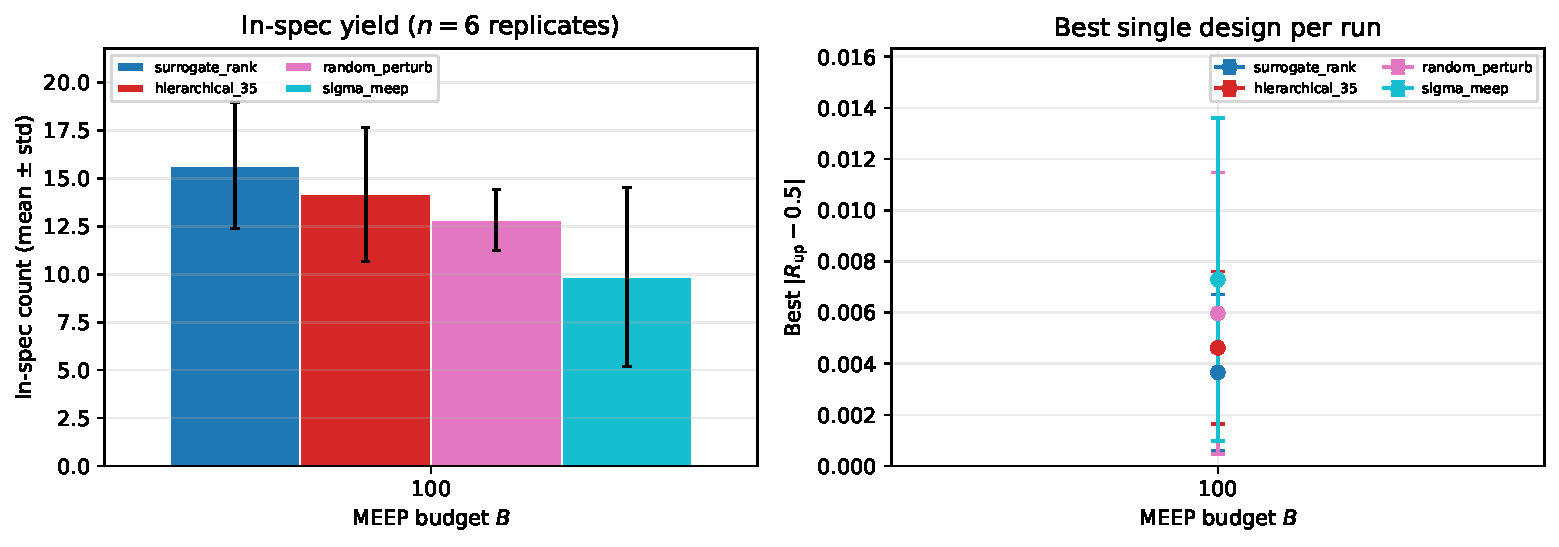
\includegraphics[width=\linewidth]{figures/sim_budget_replication_errorbars.pdf}
  \caption{Sim-budget replication ($n=6$ seeds): in-spec count vs.\ MEEP budget $B$ with 95\% CI half-widths for six search policies.}
  \label{fig:budget}
\end{figure}

\subsection{Validated positive results (release panel)}
\label{sec:positive}

Before discussing open engineering items, Table~\ref{tab:release_positive} summarizes checks that support \emph{split-ratio} promotion under the frozen contract at 1550\,nm.
These are internally consistent simulation outcomes, not claims of deployable device performance.

\begin{table}[t]
  \centering
  \caption{Release panel: outcomes that support MEEP-gated promotion (six-seed budget = pilot).}
  \label{tab:release_positive}
  \begin{tabular}{ll}
    \toprule
    Check & Outcome \\
    \midrule
    Split @ 1550\,nm ($|R_{\mathrm{up}}-0.5|\le 0.05$) & 5/5 champions pass \\
    SDF mesh audit $R_{\mathrm{up}}$ @ r25--r75 & 0.500 flat (all panel + extended) \\
    Sim-budget $B{=}100$ in-spec mean & \texttt{surrogate\_rank} highest ($15.7\pm 3.3$) \\
    Sim-budget $B{=}100$ best $|R_{\mathrm{up}}-0.5|$ & \texttt{surrogate\_rank} lowest ($0.0037\pm 0.0030$) \\
    Proposal-pool top-20 in-spec (rank vs.\ random) & 15\% vs.\ 10\% (+29\% enrichment) \\
    Fab stress nominal & 5/5 in-spec \\
    \bottomrule
  \end{tabular}
\end{table}

\section{Mesh audit and promotion gate}
\label{sec:mesh}

Split ratios computed on a pixel-staircase grid can shift with resolution, even when the underlying mask is unchanged.
Because promotion claims should not depend on a single mesh setting, we require mesh-stable cross-checks before accepting a champion.

Pixel-grid MEEP can show resolution-sensitive splits.
We promote mesh-stable cross-checks on recipe \texttt{phase0\_v1\_sdf\_geom} with \texttt{sdf\_smooth\_um = 0.04}: analytical port blocks plus signed-distance-smoothed $\varepsilon$ in the design region.
This audit recipe smooths the pixel staircase in the design island while preserving the same port frame and material constants, giving a complementary view of whether a balanced split persists across resolutions.

Dual gate for champions:
\begin{enumerate}
  \item $|\,R_{\mathrm{up}}(\text{r25}) - R_{\mathrm{up}}(\text{r50})\,| \le 0.03$
  \item $|\,R_{\mathrm{up}}(\text{r25}) - R_{\mathrm{up}}(\text{prod pixel grid})\,| \le 0.03$
\end{enumerate}
The first condition checks internal consistency of the audit recipe; the second checks agreement between audit and production discretizations.

Six champions (\texttt{local\_00022}, \texttt{meep\_bo\_00128}, \texttt{meep\_bo\_00093}, \texttt{cand\_000160}, \texttt{cand\_000003}, \texttt{cand\_000261}) pass 6/6: at 50\,px/$\mu$m all show 0.500/0.500 with zero mesh gap on the sdf recipe.
For \texttt{cand\_000261}, $|R_{\mathrm{up}}(\text{r25}) - R_{\mathrm{up}}(\text{prod})| = 0.005$.
These results support promoting the champion panel on split ratio under the stated contract.

The extended panel includes failures too: \texttt{rnd\_100\_00016\_rep02} is in-spec on the pixel grid but misses the prod-offset gate by $|{\Delta}|=0.272$.
Passing the champion audit does not imply mesh independence for arbitrary candidates---only that the promoted set behaves consistently on both recipes.

Resolution sweeps on the pixel recipe (\texttt{phase0\_v1}) show stronger mesh sensitivity than the sdf cross-check: e.g.\ \texttt{local\_00022} moves from $R_{\mathrm{up}}\approx 0.499$ at 25\,px/$\mu$m to $0.410$ at 35\,px/$\mu$m on the pixel grid while \texttt{phase0\_v1\_sdf\_geom} holds $0.500$ at the same resolutions---motivating sdf promotion rather than pixel-only claims.
Figure~\ref{fig:mesh} plots $R_{\mathrm{up}}$ vs.\ resolution for all promoted champions and extended spot-checks at 25--75\,px/$\mu$m.
Readers should interpret pixel-grid sweeps as sensitivity diagnostics and sdf-audit sweeps as the promotion-relevant stability check.

\begin{figure}[t]
  \centering
  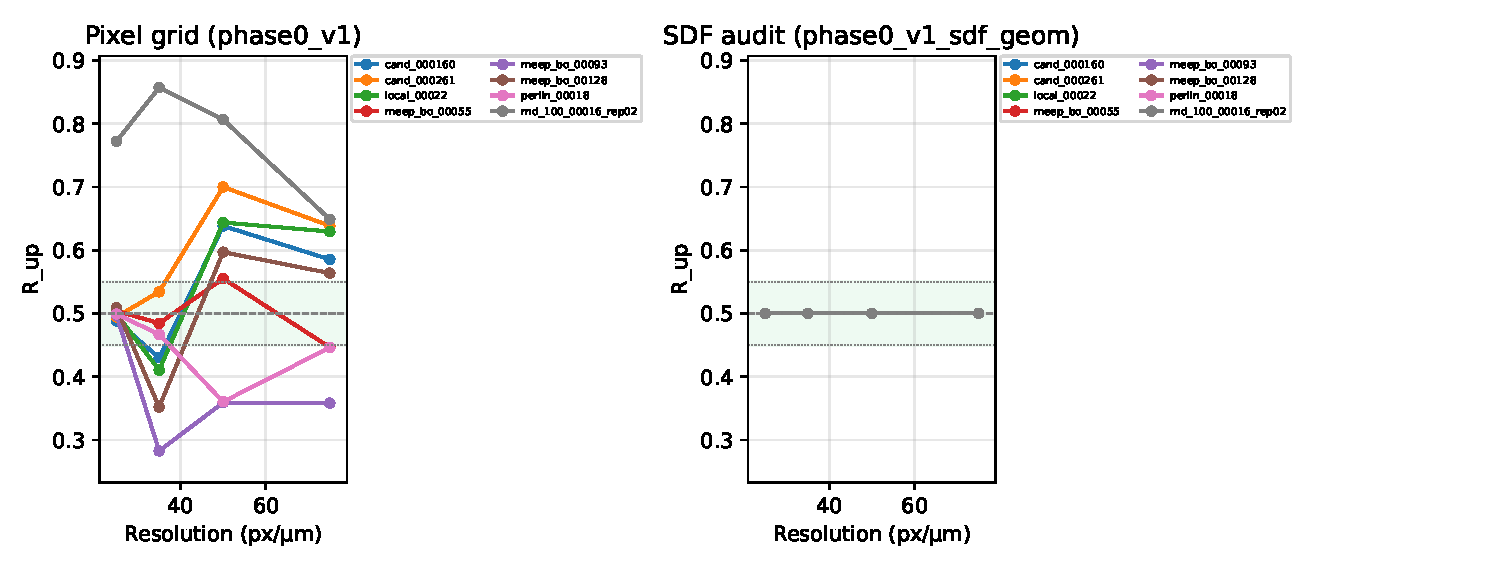
\includegraphics[width=\linewidth]{figures/champion_mesh_convergence.pdf}
  \caption{Mesh convergence on promoted designs: pixel recipe \texttt{phase0\_v1} (left) vs.\ SDF audit \texttt{phase0\_v1\_sdf\_geom} (right). Champions and extended panel; dashed lines mark $\pm 0.05$ around 0.5.}
  \label{fig:mesh}
\end{figure}

\section{Release checks: transmission, broadband, and surrogate regimes}
\label{sec:release_checks}

Promotion on split ratio at 1550\,nm is the only hard gate in Phase~0.
We therefore run additional release checks---transmission and insertion loss, wavelength dispersion, fabrication stress, and surrogate validation regimes---to document where the current recipe succeeds on that gate and where broader device targets remain open~\cite{Hansen2024BroadbandSplitters,Xing2023SpatialVariation}.

\subsection{Transmission and insertion loss}

Table~\ref{tab:champion_fom} re-simulates promoted champions on \texttt{phase0\_v1} at 1550\,nm and reports both split ratio and flux-monitor transmission metrics.
All five panel designs meet the split gate ($|R_{\mathrm{up}}-0.5|\le 0.05$) but fail proposed transmission/IL thresholds ($T_{\mathrm{total}}\ge 0.8$, IL$\le 2$\,dB): $T_{\mathrm{total}} \approx 0.01$--$0.03$ and IL$\approx 15$--$19$\,dB under the current flux-monitor normalization.
We treat these as \emph{diagnostics}, not promotion gates; split ratio remains the signed-off Phase~0 quantity.

A flux-monitor audit (\texttt{flux\_il\_audit.py}) sweeps monitor aperture height $f_y \in \{0.6,0.8,1.0,1.2\}$ (fraction of waveguide width) and input-plane offset $dx \in \{0.05,0.1,0.2\}$\,\textmu m on all five champions.
Split ratio is stable in $dx$ at fixed $f_y$ but shifts with aperture: e.g.\ \texttt{cand\_000261} reads $R_{\mathrm{up}}=0.495$ at the contract value $f_y{=}0.8$ yet $0.61$--$0.71$ at wider apertures.
Transmission is placement-sensitive---favorable monitor geometry can raise $T_{\mathrm{total}}$ from $\sim$1\% to $\sim$7\% on some designs---but IL remains $\gg 2$\,dB everywhere in the sweep.
The audit therefore does not rescue low-loss performance under this recipe; it clarifies that reported IL is not a single-point monitor bug and that $R_{\mathrm{up}}$ is defined at $f_y{=}0.8$.

\begin{table}[t]
  \centering
  \caption{Champion FOM at 1550\,nm (\texttt{phase0\_v1} r25). Split gate: $|R_{\mathrm{up}}-0.5|\le 0.05$.}
  \label{tab:champion_fom}
  \begin{tabular}{lcccc}
    \toprule
    Design & $R_{\mathrm{up}}$ & $T_{\mathrm{total}}$ & IL (dB) & Split pass \\
    \midrule
    \texttt{local\_00022} & 0.499 & 0.017 & 17.8 & yes \\
    \texttt{meep\_bo\_00128} & 0.509 & 0.031 & 15.1 & yes \\
    \texttt{meep\_bo\_00093} & 0.497 & 0.022 & 16.7 & yes \\
    \texttt{cand\_000160} & 0.488 & 0.031 & 15.1 & yes \\
    \texttt{cand\_000261} & 0.495 & 0.012 & 19.4 & yes \\
    \bottomrule
  \end{tabular}
\end{table}

\subsection{C-band dispersion}

A splitter tuned narrowly at 1550\,nm may still drift across the C-band window used in WDM systems.
We therefore sweep wavelength from 1530--1570\,nm (step 10\,nm) and apply a flatness gate requiring $|R_{\mathrm{up}}-0.5|\le 0.05$ at every sampled wavelength.

Wavelength sweeps show that single-frequency promotion does not imply flat broadband response.
Every champion passes at 1550\,nm yet fails a C-band flatness gate (worst $|R_{\mathrm{up}}-0.5|\le 0.05$ over the band): worst errors range from $0.36$ (\texttt{local\_00022}) to $0.47$ (\texttt{meep\_bo\_00128}).
Broadband hunts completed with zero verified C-band winners.
Figure~\ref{fig:broadband} overlays the five narrowband champions with the best broadband-objective verified candidate from the release hunt pool (\texttt{meep\_bo\_00162}, worst split error $0.21$); it still fails the flatness gate.
Phase~2 Perlin exploration (200 trials) reaches a best broadband objective of $0.122$ (trial 182) but has no per-wavelength MEEP curves in the release artifact and no C-band gate pass.
The takeaway is clear: Phase~0 promotion certifies balanced splitting at the design wavelength, not broadband flatness across the full C-band.

\begin{figure}[t]
  \centering
  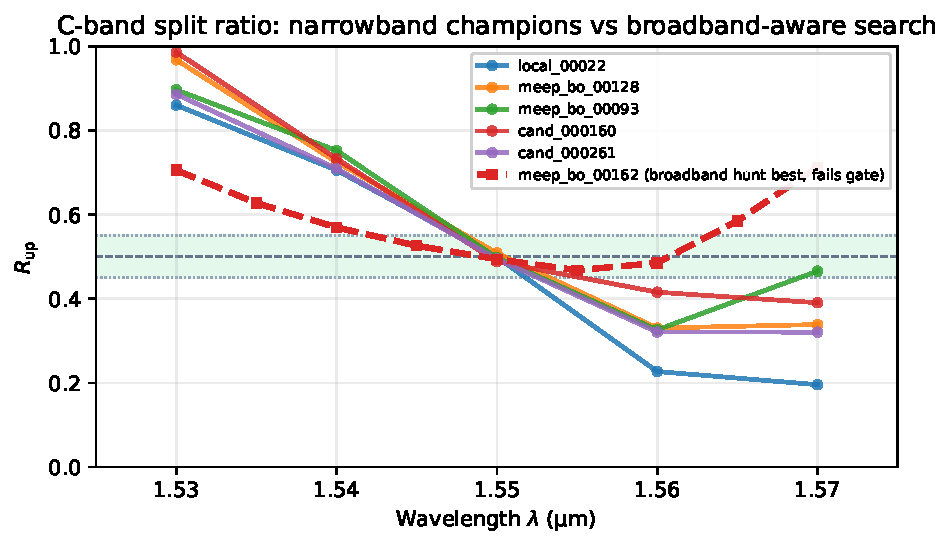
\includegraphics[width=\linewidth]{figures/broadband_contribution.pdf}
  \caption{C-band split ratio $R_{\mathrm{up}}(\lambda)$ for narrowband-promoted champions (solid) vs.\ the best broadband-aware verified candidate (dashed, fails gate). Shaded band: $|R_{\mathrm{up}}-0.5|\le 0.05$.}
  \label{fig:broadband}
\end{figure}

\subsection{Fabrication stress (binary morphology)}

Simulation-only promotion should also stress-test whether small linewidth deviations destroy the target split.
We apply binary erosion/dilation on a 5$\times$ upsampled mask grid (${\sim}$4.4\,nm/px fine pitch), stressing linewidth at nominal $\pm 10$, $\pm 20$, $\pm 30$\,nm before vote-downsampling to 180$\times$180.
This morphology test approximates over- and under-etch without running a full process simulation.

All five champions are in-spec at nominal ($|R_{\mathrm{up}}-0.5|\le 0.05$).
Under $\pm 10$--$30$\,nm binary stress on a 5$\times$ fine grid, most variants exceed $|\Delta R_{\mathrm{up}}|>0.05$ (28/30 flagged); erosion and dilation shift $R_{\mathrm{up}}$ toward channeling or upper-arm dominance.
Two dilate-30\,nm cases remain within the split gate (\texttt{local\_00022}, \texttt{meep\_bo\_00093}), showing stress response is design-dependent rather than uniformly catastrophic.
Morphology-robust latent search (\texttt{morph\_robust\_search.py}) completed with zero gate passes.
Tier~1 (240 trials, $\pm$10--20\,nm stress) yields 0/240 pass; best worst-case split error $\approx 0.389$.
Phase~2 morph hunt (277 trials) also yields 0/277 pass with best worst-case error $\approx 0.092$.
Figure~\ref{fig:fab} summarizes $R_{\mathrm{up}}$ vs.\ stress level.

\begin{figure}[t]
  \centering
  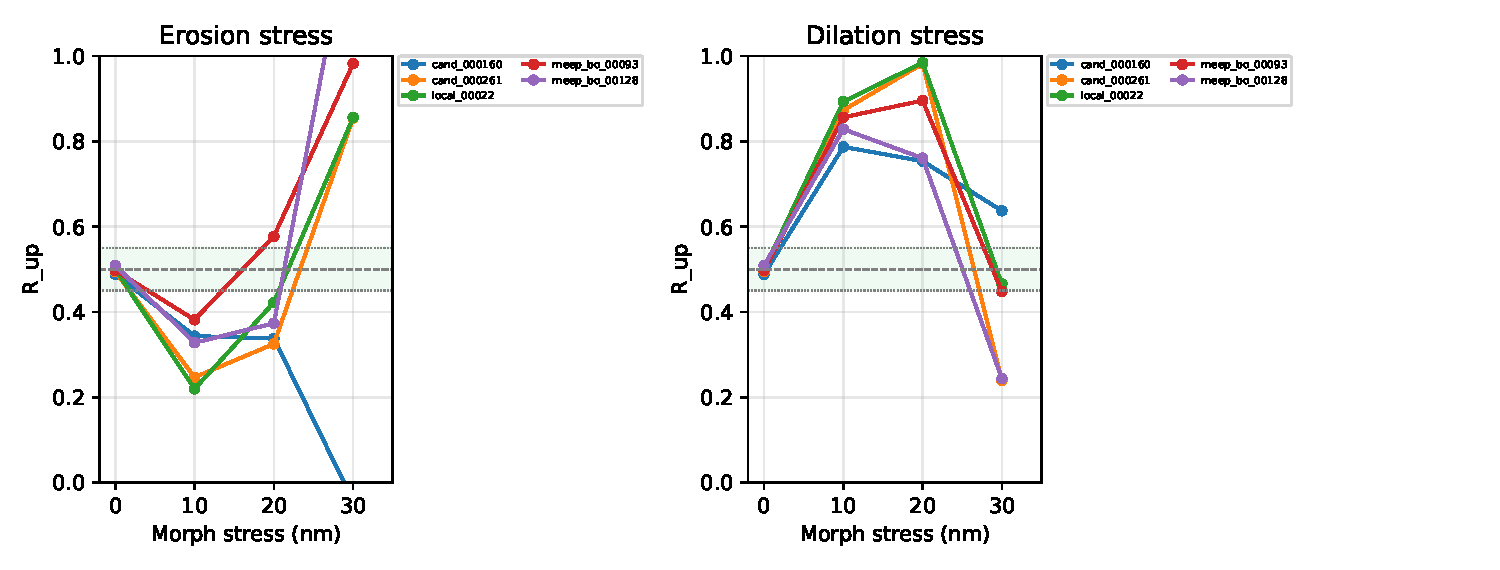
\includegraphics[width=\linewidth]{figures/champion_fab_stress.pdf}
  \caption{Fabrication stress via binary morphology (5$\times$ fine grid): erosion (left) and dilation (right) vs.\ nominal split at 1550\,nm.}
  \label{fig:fab}
\end{figure}

\subsection{Loss-aware search (split + IL objective)}
\label{sec:loss_aware}

After the flux-monitor audit, we run two IL-inclusive campaigns under the same frozen recipe.

\textbf{Phase B (champion-centered).}
Residual Optuna refinement with \texttt{objective=multi} and $\mathrm{weight\_il}{=}0.15$ (120 trials, four champion latents).
Among split-in-spec trials, best IL improves from 19.4\,dB (\texttt{cand\_000261}) and 17.8\,dB (\texttt{local\_00022}) to \textbf{17.7\,dB} at $|R_{\mathrm{up}}-0.5|{=}0.011$ (\texttt{loss\_local\_00022\_018}); split error can still reach 0.0002 at 19.4\,dB IL.
See \texttt{data/phase1/release/loss\_aware\_hunt.md}.

\textbf{Phase 2 (Perlin/sigma seeds, $\mathrm{weight\_il}{=}0.75$).}
Stage~1: 100 Perlin/$\sigma$ seeds; 15/100 in-spec at 1550\,nm.
Stage~2: IL-focused residual refine on the five lowest-IL stage-1 seeds (150 trials).
The lowest-IL design reaches \textbf{6.7\,dB} simulated IL but $|R_{\mathrm{up}}-0.5|{\approx}0.076$ (outside the split gate).
The best \emph{in-spec} Phase~2 point is 8.2\,dB IL at $|R_{\mathrm{up}}-0.5|{=}0.025$ (Perlin seed \texttt{il2\_s1\_0094}).
Artifacts: \texttt{data/phase1/release/phase2\_il\_hunt.md}.

We treat these IL numbers as flux-monitor diagnostics under \texttt{phase0\_v1}, not foundry insertion loss.
They show that IL can be driven down when the objective demands it, at a measurable split penalty on the extreme point.

\begin{figure}[t]
  \centering
  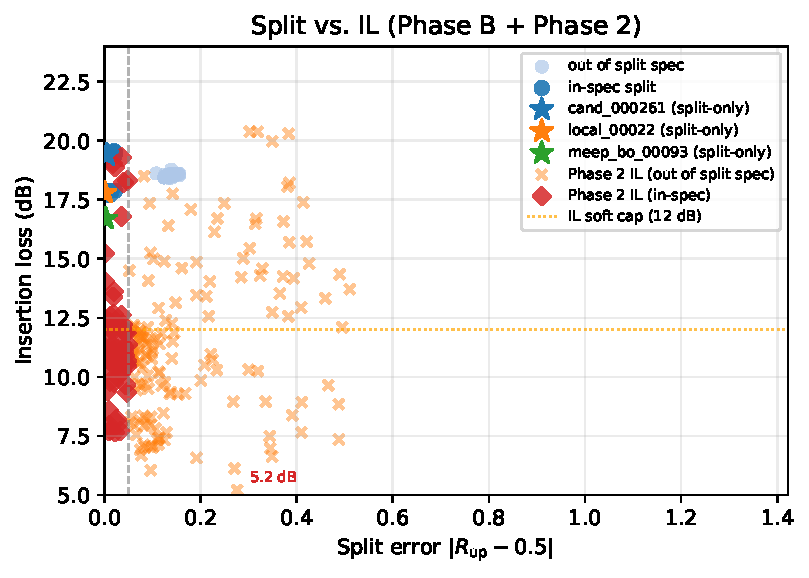
\includegraphics[width=0.72\linewidth]{figures/loss_aware_tradeoff.pdf}
  \caption{Split error vs.\ insertion loss: Phase~B loss-aware trials (blue), Phase~2 IL hunt (orange/red), and split-only champions (stars). Vertical dashed line: split gate; horizontal dotted line: 12\,dB soft IL cap in Phase~B.}
  \label{fig:loss_tradeoff}
\end{figure}

\subsection{Surrogate validation regimes}

Surrogate quality depends on how the holdout set is constructed.
We report three holdout regimes on the merged corpus (Table in \texttt{surrogate\_validation.md}): random 80/20 ($R^2\approx -9$ on $|R_{\mathrm{up}}-0.5|$), $\sigma$-grouped holdout ($R^2\approx -11$), and chronological train-pre-AL / test-gated-shortlist ($R^2\approx -89$, $n_{\mathrm{val}}{=}25$).
Spearman on $|R_{\mathrm{up}}-0.5|$ is $\sim$0.40--0.46 under random and grouped splits; ranking top-20 by surrogate error does not beat an oracle random top-20 on held-out \emph{absolute} error in these snapshots.

The $\sigma$-grouped diagnostic ($R^2\approx 0.45$ on $|R_{\mathrm{up}}-0.5|$ elsewhere in this work) remains the intended regression sanity check when perturbation balls do not leak between train and validation.
Even there, MEEP shortlist outcomes are the promotion metric: a surrogate is useful if it improves verified yield at fixed budget, not if it wins a random holdout on absolute split error.

\section{Discussion}
\label{sec:discussion}

This study establishes a reproducible \emph{search pattern}---manifold sample, surrogate rank, MEEP verify, corpus append---and pilots it on one gate: balanced split at 1550\,nm under \texttt{phase0\_v1}.
The positive result is budget efficiency for that gate, not a finished splitter product.
Adopters can reuse the pattern while swapping gates (broadband flatness, robust morphology, IL) and forward models; \S\ref{sec:roadmap} outlines concrete next steps and points to open artifacts.

\subsection{Why ranking beats $R^2$ here}

The label distribution is heavy-tailed in split error: most random manifold samples are far from 0.5.
MSE regression chases a poorly identified conditional mean; pairwise rank loss~\cite{Burges2010LambdaRank} aligns with the verification decision rule (sort candidates, MEEP the top few).
Negative val $R^2$ under a random 80/20 holdout is therefore unsurprising and should not be reported as a product metric~\cite{Jiang2021SurrogateReview}.
With $\sigma$-grouped validation (no leakage across perturbation balls), predicting $|R_{\mathrm{up}}-0.5|$ reaches val $R^2 \approx 0.45$ on the merged corpus---still a diagnostic, not a promotion gate.
For reporting we use Spearman on $|R_{\mathrm{up}}-0.5|$, top-$k$ in-spec counts, and MEEP outcomes on gated shortlists.
MAPS~\cite{MAPS2025}, CNN-IBO~\cite{SciRep2025CNNIBO}, and neural-operator surrogates~\cite{Frenkel2023NeuralOperator} attack similar budget-allocation problems in adjoint or surrogate-accelerated loops; here the emphasis is a fixed MEEP contract on a DRC manifold with explicit per-budget yield accounting.

\subsection{Relation to differentiable inverse design}

Danis \emph{et al.}~\cite{Danis2026DRCManifold} optimize through differentiable DRC manifolds end-to-end; we stop at MEEP-verified promotion on a frozen recipe.
Our Track~C experiments wire champions into invrs-gym's Ceviche lightweight power-splitter challenge~\cite{Christiansen2024InvrsGym,Fan2019Ceviche,Schubert2022CevicheChallenges} (lower eval metric is better; in-spec when $\mathrm{eval\_metric} \ge 0$):
\begin{itemize}
  \item Gym-native density L-BFGS reaches in-spec metrics $\sim$0.058 (best history step) vs.\ $\sim$0.092 final after 200 steps.
  \item Latent refinement through \texttt{decode\_soft} on MEEP champions beats the published leaderboard entry ($0.0090$): best in-spec metrics are $0.0010$ (\texttt{meep\_bo\_00128}), $0.0012$ (\texttt{local\_00022}), and $0.0060$ (\texttt{meep\_bo\_00093}) at 120 Adam steps (lr $=0.02$).
  \item MEEP \texttt{phase0\_v1} promotion diverges: gym loss is not interchangeable with our frozen FDTD recipe (different cell size, 1.6\,$\mu$m vs.\ 4\,$\mu$m design region, FDFD vs.\ MEEP).
\end{itemize}
Track~C is useful for checking that gradients flow through the decoder; it does not replace MEEP gates.

\subsection{Limitations and open engineering items}

We close with an explicit accounting of what this study does and does not establish.
Each limitation below is tied to a concrete future-work item for adopters extending this pattern.

\begin{enumerate}
  \item \textbf{2D TE effective-index model.} All promotion numbers use a 2D TE simulation without full 3D vectorial slab dispersion or fabrication corner rounding beyond the sdf audit.
  \emph{Future work:} 3D MEEP or foundry PDK cross-check before any absolute performance claim~\cite{Hansen2024BroadbandSplitters}.
  \item \textbf{Fixed ports and template.} Masks optimized for other topologies may not map cleanly to this 1$\times$2 frame; \texttt{mask\_flip\_y} is part of the contract, not a universal physical fix.
  \emph{Future work:} re-derive the contract per topology or port frame before comparing to literature devices~\cite{Piggott2017InverseDesign}.
  \item \textbf{Heuristic DRC.} EBeamModel rules are not a foundry sign-off; optical spec and DRC spec are decoupled.
  \emph{Future work:} integrate lithography or etch models into the search loop~\cite{Faid2024FabricationAware,Schubert2022CevicheChallenges}.
  \item \textbf{No fab validation.} We report simulation-only splits; no correlation to measured wafer data is available.
  \emph{Future work:} layout-aware Monte Carlo with spatial process maps~\cite{Xing2023SpatialVariation} and flux-monitor calibration against reference structures.
  \item \textbf{Pilot policy comparison ($n{=}6$).} Surrogate rank leads or ties at $B{=}100$ (3/6 paired wins vs.\ hierarchical\_35), not at $B{=}30$; larger replication is needed for definitive policy ordering.
  \emph{Future work:} expand to $n{\ge}20$ seeds with frozen corpus and paired-win reporting.
  \item \textbf{Narrowband promotion.} Champions are 50/50 at 1550\,nm but dispersive over 1530--1570\,nm (0/39 verified candidates pass a C-band flatness gate).
  \emph{Future work:} multi-wavelength objectives and per-$\lambda$ MEEP verification as in broadband inverse-design practice~\cite{Hansen2024BroadbandSplitters,Piggott2017FabricationConstrained}.
  \item \textbf{Morphology fragility.} Binary $\pm 10$--$20$\,nm pixel stress breaks most champions; 0/517 morph-refine trials pass combined gates.
  \emph{Future work:} variation-aware or fabrication-tolerant optimization~\cite{Piggott2017FabricationConstrained,BOSON2024,Wolff2024FabricationTolerant} with stress in the inner loop, not post-hoc filtering.
  \item \textbf{Flux-monitor IL.} Reported $T_{\mathrm{total}}$ and IL are diagnostics under uncorrected flux normalization ($T_{\mathrm{total}}\sim 0.01$--$0.03$); the 6.7\,dB Phase~2 point fails the split gate.
  \emph{Future work:} reference-waveguide calibration and IL in the promotion objective once monitors are anchored~\cite{Xing2023SpatialVariation,Hughes2018AdjointNonlinear}.
  \item \textbf{Incomplete mesh independence.} Champion panel passes on sdf audit; pixel-grid resolution sweeps remain sensitive.
  \emph{Future work:} sdf-based promotion as default gate; document pixel-grid sensitivity as diagnostic only.
\end{enumerate}

\section{Conclusion}
\label{sec:conclusion}

We present a starting point for MEEP-gated inverse design on DRC-feasible manifolds: a reproducible loop in which a ranking surrogate narrows candidates and MEEP alone promotes them under a frozen \texttt{phase0\_v1} contract.
On the single gate tested here---balanced split at 1550\,nm---a six-seed pilot shows surrogate-ranked search improves verified in-spec yield per simulation dollar vs.\ random perturbation and $\sigma$-only MEEP BO at $B{=}100$, while hierarchical $\sigma$ policies remain competitive (paired tie 3/6).
The corpus, configs, and release artifacts are open for others to rerun or extend.

Equally important are the diagnostic negatives documented under the same contract: narrowband promotion does not yield C-band flatness; promoted masks are morph-fragile; flux-monitor IL and transmission remain poor and uncalibrated.
Those results define the boundary of the present recipe and invite adopters to test whether the same search pattern helps once gates, objectives, and fabrication models are upgraded---as outlined in \S\ref{sec:roadmap}.

\section{Next steps for adopters}
\label{sec:roadmap}

We intend this preprint as an invitation to build on a \emph{pattern}, not a product release.
The pattern---manifold sample $\to$ surrogate rank $\to$ MEEP verify $\to$ corpus---proved useful for one gate (split at design $\lambda$).
Others can ask whether it transfers to broadband WDM flatness, morphology robustness, IL/transmission, or different splitter topologies by changing the gate while keeping budget accounting honest.

\paragraph{Adoption checklist.}
\begin{enumerate}
  \item \textbf{Freeze the forward-model contract.} Pin recipe ID, resolution, port frame, polarization, and monitor placement; version-label every label row (\texttt{recipe\_version}).
  \item \textbf{Define promotion gates explicitly.} Separate narrowband split, C-band flatness, IL/$T$, and morphology stress; do not promote on surrogate scores alone~\cite{Jiang2021SurrogateReview,Frenkel2023NeuralOperator}.
  \item \textbf{Refresh the surrogate on the corpus.} Retrain ranking models as verified rows accumulate; report Spearman on $|R_{\mathrm{up}}-0.5|$ and top-$k$ enrichment, not holdout $R^2$ alone.
  \item \textbf{Account MEEP budget per policy.} Compare methods at matched $B$ with paired seed wins; log $M$ proposals vs.\ $B$ verifications.
  \item \textbf{Close the sim--fab gap deliberately.} For foundry-facing claims, add layout-aware variability maps or fabrication-aware inverse design~\cite{Xing2023SpatialVariation,Faid2024FabricationAware,BOSON2024} rather than extrapolating from uncorrected flux monitors.
\end{enumerate}

\paragraph{Translation paths by target.}
For \textbf{broadband splitters}, multi-wavelength objectives with per-$\lambda$ verification follow established inverse-design practice~\cite{Hansen2024BroadbandSplitters,Piggott2017FabricationConstrained}.
For \textbf{morphology robustness}, erosion/dilation stress should move into the optimization inner loop via fabrication constraints or variation-aware subspace methods~\cite{Piggott2017FabricationConstrained,Wolff2024FabricationTolerant,BOSON2024}.
For \textbf{IL and transmission}, adjoint or multi-objective loops with calibrated monitors are the natural upgrade path~\cite{Hughes2018AdjointNonlinear,Hammond2022MeepAdjoint}; our Phase~2 hunt shows split--IL tradeoffs even before calibration.
For \textbf{surrogate-accelerated search}, neural-operator or CNN surrogates can replace our mask MLP while preserving MEEP as promotion authority~\cite{Frenkel2023NeuralOperator,Su2021DeepSurrogate,SciRep2025CNNIBO}.

\paragraph{Open artifacts.}
Source code, scripts, and corpus layout are public at \url{https://github.com/pberlizov/nanophotonics-inverse-design} (MIT license).
MEEP label corpora and release summaries are under \texttt{data/phase0/} and \texttt{data/phase1/release/} in that repository; large FDTD outputs are gitignored and mirrored in the Zenodo bundle.
The Zenodo deposit mirrors \texttt{manuscript.pdf}, figures, release markdown summaries, \texttt{CITATION.cff}, and \texttt{repro\_manifest.json} for citation-stable reuse.

\section*{Data and code availability}

All code and configuration are at \url{https://github.com/pberlizov/nanophotonics-inverse-design}.
Corpus labels, sim-budget replicates, novelty metrics, and promotion checks live under \texttt{data/phase0/} and \texttt{data/phase1/} (regenerate locally or use the Zenodo bundle for frozen release summaries).

\appendix
\section{Recipe parameter table}
\label{app:recipe}

\begin{table}[h]
  \centering
  \caption{Full Phase~0 MEEP recipes.}
  \label{tab:full-recipe}
  \small
  \begin{tabular}{lll}
    \toprule
    Key & \texttt{phase0\_v1} (prod) & \texttt{phase0\_v1\_sdf\_geom} (audit) \\
    \midrule
    Backend & MEEP 2D TE & MEEP 2D TE \\
    Resolution & 25 / 50 px/$\mu$m & 25 / 50 px/$\mu$m \\
    Cell size & 6\,$\mu$m & 6\,$\mu$m \\
    Design region & 4\,$\mu$m & 4\,$\mu$m \\
    Mask size & 180$\times$180 & 180$\times$180 \\
    \texttt{mask\_flip\_y} & true & true \\
    $w_g$ & 0.45\,$\mu$m & 0.45\,$\mu$m \\
    PML & 0.5\,$\mu$m & 0.5\,$\mu$m \\
    $\varepsilon_{\mathrm{Si}}$ / $\varepsilon_{\mathrm{SiO}_2}$ & 12.0 / 2.25 & 12.0 / 2.25 \\
    Design $\varepsilon$ & pixel staircase & SDF smooth, 0.04\,$\mu$m \\
    Source & Gaussian $Ez$, $f=1/1.55$ & same \\
    Run termination & flux decay $10^{-4}$ & flux decay $10^{-4}$ \\
    Promotion gate & in-spec @ r25 & $|{\Delta}R|_{25,50}\le 0.03$, \\
    & & $|{\Delta}R|_{\mathrm{prod,sdf}}\le 0.03$ \\
    \bottomrule
  \end{tabular}
\end{table}

Surrogate training defaults: \texttt{mask\_mlp}, hidden [256,128,64], \texttt{mask\_pool=6}, $\sigma$ feature enabled, sources \texttt{perturb\_plus\_search}, champion-weighted sampling.
Rank model: \texttt{loss\_mode=pairwise\_rank} (\texttt{surrogate\_improved\_rank}).

\bibliographystyle{unsrt}
\bibliography{refs}

\end{document}
